\section{Introduction}
\dropcap{S}oft robotic development is inherently complex, requiring the seamless integration of materials, geometry, actuation, and sensing with compliant continuum dynamics, perception, and control systems. Co-design strategies have proven effective in addressing multi-objective problems and accommodating the compositional, hierarchical nature of complex systems~\citep{zardini2023co}, thereby potentially allowing for finding the delicate balance between safety and performance. Successful co-design has been demonstrated in fields such as chemistry~\citep{norskov2009towards,vaissier2018computational}, construction engineering~\citep{knippers2021integrative}, articulated robotics~\citep{ha2018computational,zhao2020robogrammar}, and self-driving vehicles~\citep{zardini2021co}.
% 
Recent research has begun to develop co-design algorithms for soft robots that simultaneously optimize the body (e.g., morphology) and the brain (e.g., control and perception systems)~\citep{van2018spatial, spielberg2019learning, chen2020design, bhatia2021evolution, spielberg2021co, wang2023preco, medvet2021biodiversity, wang2022curriculum, junge2022leveraging, legrand2023reconfigurable, wang2024diffusebot, navez2024contributions}. However, several shortcomings limit their broader application. First, the optimization cycles are computationally expensive, hindering full design space exploration and global optimum identification, thus reducing practical utility~\citep{chen2020design}. This inefficiency arises from high-dimensional design spaces (e.g., voxel- or particle-based discretizations)~\citep{spielberg2019learning, medvet2021biodiversity, medvet2022impact, wang2022curriculum, legrand2023reconfigurable, wang2023softzoo, wang2023preco, wang2024diffusebot}, inefficient optimization routines (e.g., evolutionary algorithms)~\citep{chen2020design, rieffel2014growing, hiller2012automatic, bhatia2021evolution, medvet2021biodiversity, medvet2022impact}, and expensive control derivation via inner loops where a \gls{RL} controller is trained from scratch for each iteration~\citep{bhatia2021evolution, wang2022curriculum, wang2023softzoo, wang2023preco}, compounded by the reliance on computationally intensive simulations for evaluating the fitness of a design~\citep{spielberg2019learning, medvet2021biodiversity, medvet2022impact, wang2022curriculum, legrand2023reconfigurable, wang2023softzoo, wang2023preco, wang2024diffusebot}.
% 
Second, a narrow focus on easily computable evaluation metrics (e.g., locomotion speed, workspace) often neglects other vital design values such as usability, safety, cost, ecological impact, and regulatory requirements~\citep{junge2022leveraging}. For example, manufacturability is frequently overlooked, leading to voxel-based designs that are rarely practical to fabricate~\citep{legrand2023reconfigurable, wang2024diffusebot}.
% 
Third, evaluation metric uncertainty is seldom addressed~\citep{chen2020design}, resulting in designs that perform well in simulation but underperform in real-world scenarios.
% 
Finally, current co-design methods generally fail to incorporate diverse stakeholder input or account for end-user requirements.

The holistic co-design framework proposed in this chapter adopts a comprehensive view of design values and components, offering a path to address previous shortcomings of soft robotic co-design through several key modifications. First, it considers a wide range of requirements, objectives, and constraints—including safety, fabrication and operation costs, environmental impact, and regulatory restrictions. Second, we introduce enhancements to computational co-design that can significantly boost efficiency by (i) embracing reduced-order design spaces from which designs are sampled and decoded into full spatial morphologies~\citep{wang2024diffusebot}; (ii) co-optimizing reduced-order dynamical models—whether physics-based~\citep{armanini2023soft} or learned~\citep{liu2024physics, alkayas2025soft, stolzle2024input, valadas2025learning, navez2025modeling}—to capture the specific deformations experienced during tasks while minimizing model complexity; (iii) employing less expensive auxiliary metrics (e.g., controllability or observability based on the reduced-order model) that provide early feedback to eliminate likely underperforming designs; and (iv) replacing RL controllers trained from scratch with existing, more efficient model-based control techniques that exploit the reduced-order model~\citep{della2023model, stolzle2024input}. Third, we take a probabilistic view on co-design, acknowledging that evaluation metrics can be uncertain—due, for example, to the sim-to-real gap~\citep{dubied2022sim}—but that high-fidelity simulations and prototyping at varying \glspl{TRL}~\citep{NASA_TRL} can reduce this uncertainty. We formalize the tradeoff between "refinement" (computational optimization based on current metric beliefs) and "realization" (prototyping a design and acquiring true measurements for the evaluation metrics), paving the way for a resource-efficient holistic co-design strategy. Finally, early stakeholder involvement through structured consultations and iterative feedback ensures that practical insights on usability, manufacturability, and scalability are integrated, aligning design decisions with real-world criteria.

\begin{figure}[tb]
    \centering
    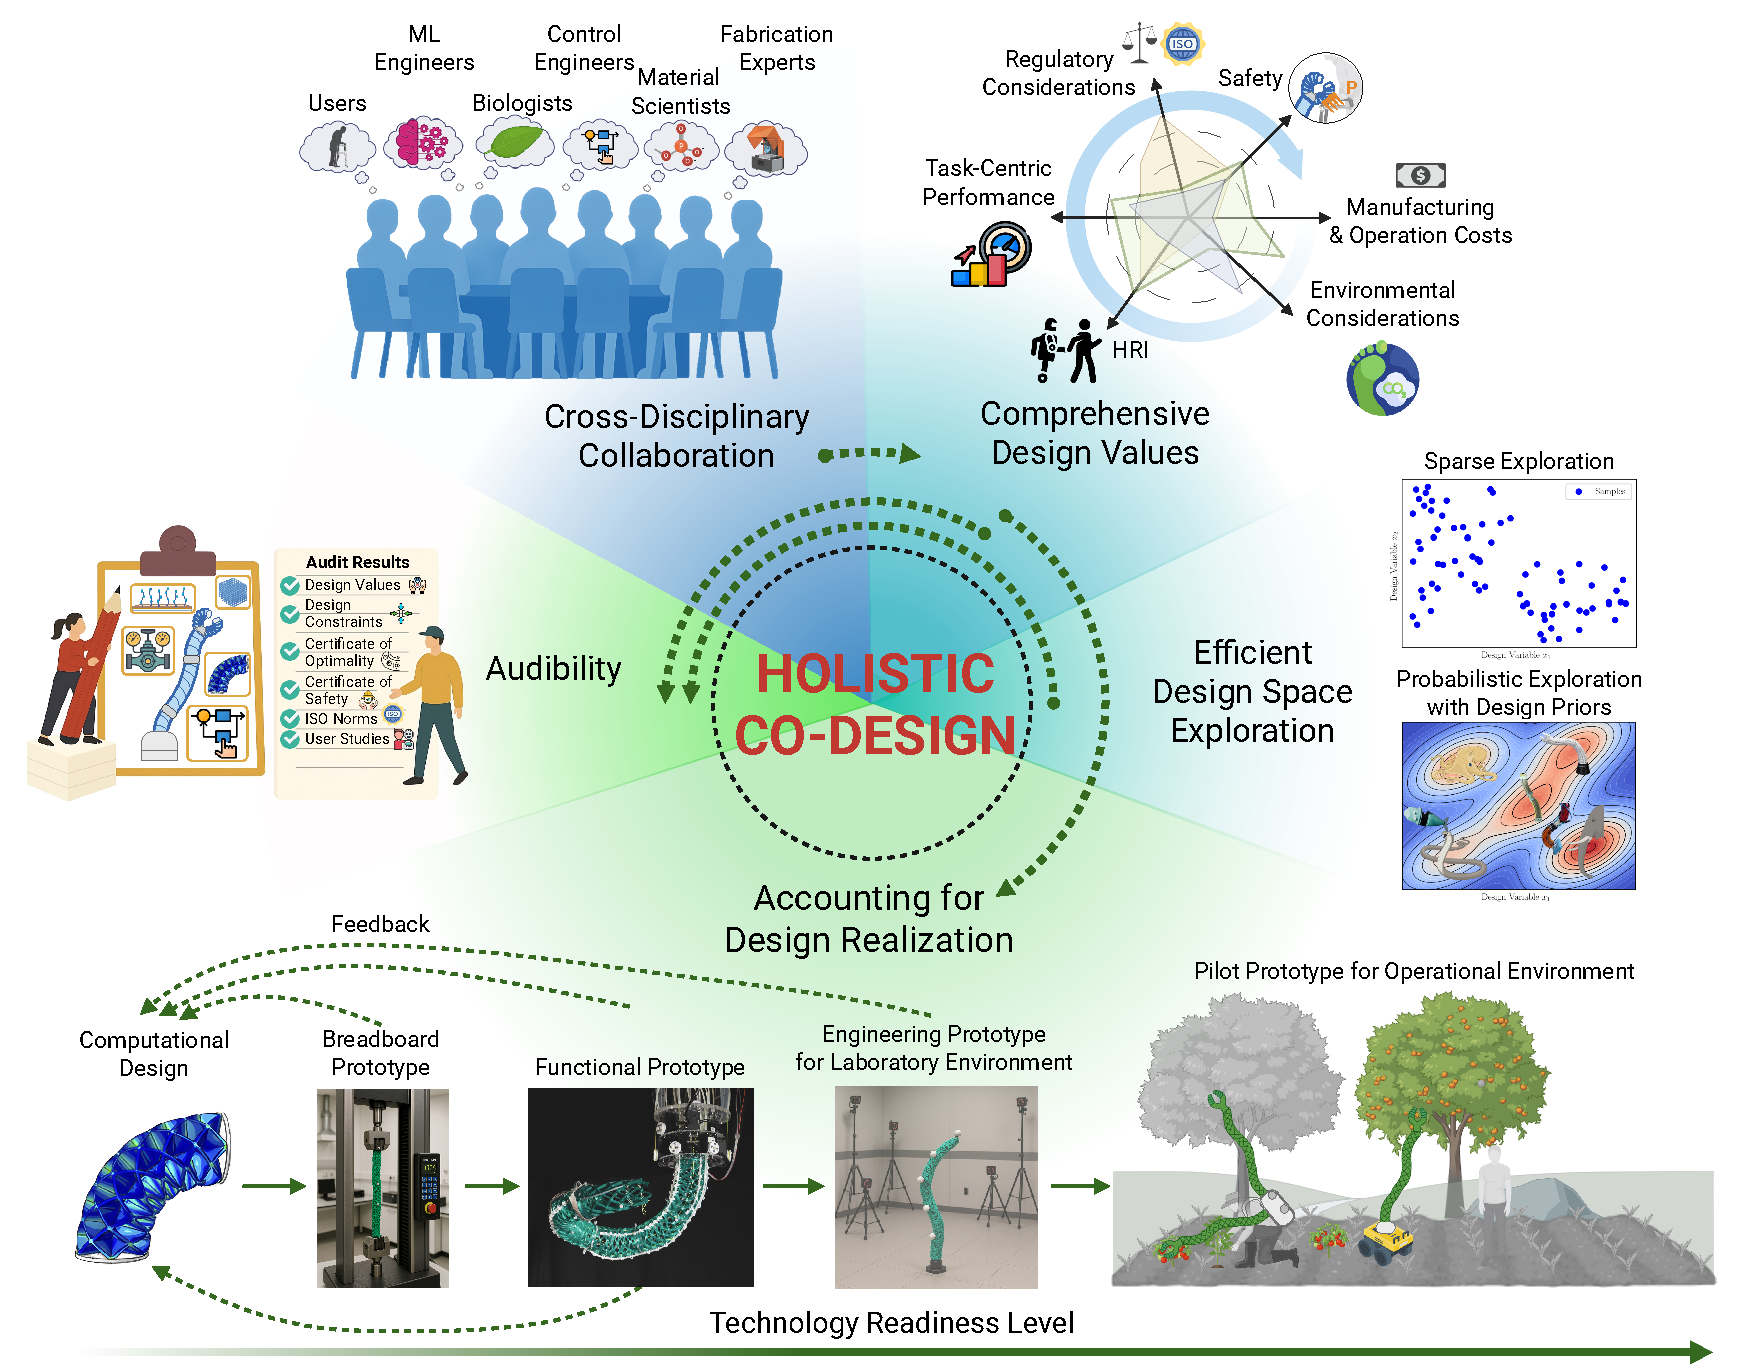
\includegraphics[width=\textwidth]{appendix-holistic-codesign/figures/holistic_codesign_overview_layered.pdf}
    \caption{
    \textbf{Holistic Co-Design of Soft Robots.}
    The five pillars of holistic co‑design are (1) Incorporating comprehensive design requirements and values directly into multi‑objective optimization; (2) Efficiently exploring the full design space by melding design priors (e.g., biological inspirations, existing solutions) with computationally efficient co‑design routines; (3) Explicitly accounting for design realization (e.g., prototyping and testing) via a probabilistic treatment of evaluation metrics and by formalizing the refinement‑vs‑realization trade‑off—enabling targeted prototyping to reduce metric uncertainty and narrow the sim‑to‑real gap; (4) Fostering cross‑disciplinary collaboration and involving all relevant stakeholders in defining design values and providing iterative feedback; (5) Ensuring auditability to preserve design knowledge and guarantee reproducibility.
    These pillars are inherently interconnected (see green arrows)—for example, stakeholders and the design team co‑define design requirements, certain design values (e.g., HRI) demand evaluation in the real world (i.e., enabled by realization), and both the exploration of the design space and the fulfillment of design requirements remain fully auditable.
    }
    \label{fig:apx:holisticcodesign:overview}
\end{figure}

Illustrated in Fig.~\ref{fig:apx:holisticcodesign:overview}, this holistic co-design framework for soft robots has the potential to reshape societal norms by empowering robots to take on critical roles in caregiving, education, and other sensitive fields. By deploying more effective and high-performing soft robots in human-centric environments while ensuring the necessary safety, we can enhance human well-being, address key societal challenges, and foster broader societal acceptance of robots.